%%%%%%%%%%%%%%%%%%%% author.tex %%%%%%%%%%%%%%%%%%%%%%%%%%%%%%%%%%%
%
% sample root file for your "contribution" to a proceedings volume
%
% Use this file as a template for your own input.
%
%%%%%%%%%%%%%%%% Springer %%%%%%%%%%%%%%%%%%%%%%%%%%%%%%%%%%

%8 à 10 pages (12 avec biblio)


\documentclass{svproc}
\usepackage{amsmath}
\usepackage{cleveref}
%
% RECOMMENDED %%%%%%%%%%%%%%%%%%%%%%%%%%%%%%%%%%%%%%%%%%%%%%%%%%%
%

%tikz 
\usepackage{tikz}
\usepackage{pgfplots}
\usepackage{amsmath}
\usetikzlibrary{decorations.pathmorphing, positioning}
\definecolor{echoreg}{HTML}{2cb1e1}
\definecolor{echodrk}{HTML}{0099cc}
\tikzstyle{mybox} = [text=black, very thick,
    rectangle, rounded corners, inner sep=10pt, inner ysep=20pt]
\tikzstyle{fancytitle} =[text=black]
\newcommand{\yslant}{0.5}
\newcommand{\xslant}{-0.6}
%%%%%%%%%%%%%%%%%%%%%%%%%%%%%%%% TIKZ STYLES
\tikzstyle{every node}=[font=\scriptsize]

\tikzset{RootStyle/.style = {
						shape          = circle,
			      draw           = red!50!black!50,
			      thick,
			      top color      = white,
			      bottom color   = red!50!black!20,
			      text           = black,
			      inner sep      = .2pt,
			      outer sep      = 0pt,
			      minimum size   = 2.5 mm}
						}

\tikzset{VertexStyle/.style = {
						shape          = circle,
			      draw           = black!50,
			      top color      = white,
			      bottom color   = black!20,
			      text           = black,
			      inner sep      = .2pt,
			      outer sep      = 0pt,
			      minimum size   = 8 mm}
						}

\tikzset{EdgeStyle/.style   = {thick,-}}

\tikzset{LabelStyle/.style =   {
				  text           = black,
				  inner sep      = .2pt,
				  outer sep      = 1pt,
				  font           =\scriptsize,
				  minimum size   = 2.15 mm}
					}

\pgfplotsset{compat=1.15}

\newcommand\overmat[3]{%
  \makebox[0pt][l]{$\smash{\color{#3}\overbrace{\phantom{%
    \begin{matrix}#2\end{matrix}}}^{\text{#1}}}$}#2}
\newcommand\undermat[3]{%
  \makebox[0pt][l]{$\smash{\color{#3}\underbrace{\phantom{%
    \begin{matrix}#2\end{matrix}}}_{\text{#1}}}$}#2}
\newcommand\partialphantom{\vphantom{\frac{\partial e_{P,M}}{\partial w_{1,1}}}}

% to typeset URLs, URIs, and DOIs
\usepackage{url}
\def\UrlFont{\rmfamily}


\begin{document}
\mainmatter              % start of a contribution
%
\title{Different centralities in multilayer stream graphs}
%
\titlerunning{Centralities in Multilayer stream graphs}  % abbreviated title (for running head)
%                                     also used for the TOC unless
%                                     \toctitle is used
%
\author{Pimprenelle Parmentier\inst{1} \and Tiphaine Viard\inst{1}
Jean-François Baffier\inst{2} \and Benjamin Renoust\inst{3}}
%
\authorrunning{Pimprenelle Parmentier et al.} % abbreviated author list (for running head)
%
%%%% list of authors for the TOC (use if author list has to be modified)
\tocauthor{Pimprenelle Parmentier, Tiphaine Viard, Jean-François Baffier, Benjamin Renoust}
%
\institute{RIKEN AIP, Tokyo, Japan
\and
Japan Society for the Promotion of Sciences
\and 
Institute for Datability Science, Osaka Univerisity}

\maketitle              % typeset the title of the contribution

\begin{abstract}
Graphs are commonly used in mathematics to represent some relationships between items. We generalise this model to networks of relationships which have complex structure and which depend on the time and we build and test several ``centralities'' to catch the importance of nodes, links and layers of such structures. We compare our new notions with the traditional ones. To illustrate this notions, we give example of use on US flights dataset and a network of different type of relationships between students.
%The abstract should summarize the contents of the paper using at least 70 and at most 150 words. It will be set in 9-point font size and be inset 1.0 cm from the right and left margins. There will be two blank lines before and after the Abstract. \dots
% We would like to encourage you to list your keywords within
% the abstract section using the \keywords{...} command.
\keywords{multilayer graph, stream graph, centrality, entanglement, density}
\end{abstract}
%

\section{Introduction}
%
From the time, in 1750, that stated the bridges problem of Köninsgberg, the notion of graphs has been widely exploited to model and sort a lot of real-life and theoretical problems.

A graph represent a set of relationships (links) between entities (nodes). This type of data can be found everywhere: road or rails between cities, friendships, communications between internet devices, etc. 

This formalism has been extended to capture diversity in the data: links can be oriented, weighted, labelled, \textit{etc}. The nodes can have different labels too. The nodes and the links can change with the time. Several new formalisms have been created to deal with this new aspects. We focus on two of them: the multilayer graphs~\cite{mlkiv} to deal with non-trivial structures and the stream graphs~\cite{stream} to deal with time-dependant interactions. We use this two formalisms and the theories associated to describe time-dependant set of interactions with complex structures.

In the first part, the multilayer stream graph is constructed with its theoretical definitions. The we give example of use with to real datasets.


\section{The multilayer stream graph}
%


\subsection{Preliminaries: multilayer graphs and stream graphs}
%
An graph is a tuple $G=(V,E)$ composed by a set of nodes $V$ and a set of edges $E\subseteq V \otimes V$, where each edge is an unordered pair of two different nodes. A directed graph has a set of directed edges $E\subseteq V\times V$, where $(u,v) \neq (v,u)$.

To illustrate the definitions of all the graphs, we will use the same example: a population of monkeys $F_1, F_2, M_1, M_2$ (two females and two males). In the \cref{fig:graphsimple}, we put a link between two animals if they have been in contact.

\begin{figure}[h]
			\begin{center}
					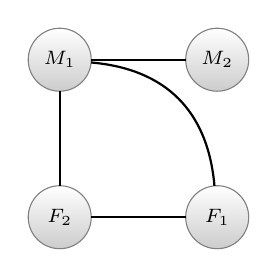
\begin{tikzpicture}[xscale=2,yscale=2,auto]
							\draw (1,0) node[VertexStyle]   (A) { $F_1$ };
							\draw (0,0) node[VertexStyle] (B) { $F_2$ };
							\draw (0,1) node[VertexStyle]   (C) { $M_1$ };
							\draw (1,1) node[VertexStyle]   (D) { $M_2$ };

							\draw[EdgeStyle]				(B) to node[LabelStyle]{}	(A);
							\draw[EdgeStyle,bend left=40,looseness=1.1]    	(C) to node[LabelStyle]{}   	(A);
							\draw[EdgeStyle] 	(C) to node[LabelStyle]{}     	(B);
							\draw[EdgeStyle]  	(C) to node[LabelStyle]{} 		(D);
							

					\end{tikzpicture}
			\end{center}
	\caption{An example of undirected graph. The nodes $V=(F_1, F_2, M_1, M_2)$ are monkeys, and the undirected edges $E=(M_1,M_2),(M_1,F_1),(M_1,F_2),(F_1,F_2)$ represent the fact that they have been in contact.}
	\label{fig:graphsimple}
\end{figure}

The {\bf degree} of a node $v\in V$ $d(v)$ is the number of edges in which $v$ is appears: $d(v)=|\{(u,w) \in E \subseteq V \otimes V| u=v \cup w=v\}|$.

\subsubsection{Multilayer graphs}
%
Imagine now that we want to describe in a more precise way the type of interaction between the monkeys. For instance, the monkey can meet in different places, like the mountain or the plain. The can have face to face relations to collaborate or to fight.

A {\em multilayer graph}~\cite{mlkiv,mldd} is a set $M=(V_M,E_M,V,{\cal L})$.\\
${\cal L}$ is the {\em structure}: it is a finite set of $d$ different sets, named {\em aspects}: ${\cal L} = L_1, \dots, L_d$. Each aspect $L_i$ contains elements $l_i^1,\dots l_i^{n_i}$ which are named {\em elementary layers}. A {\em layer} $\alpha$ is then a combination of elementary layers from each aspect: $\alpha \in L=L_1\times \dots \times L_k$. \\
$V$ is the set of nodes and each of them can be present or not on the different layers. A node on a layer is called a {\em node-layer}. The set of nodes-layers is $V_M \subseteq V \times L$. Each node-layer can be linked to another with undirected ($E_M\subseteq V_M \otimes V_M$)or directed ($E_M \subseteq V_M \times V_M$) edges.

In the monkeys example \cref{multimonkeys}, the nodes are still the monkeys. The structure is made of two aspects: the place and the type of interaction. A layer can be for instance (mountain,collaboration). They are different types of links, depending on which layer are the nodes.

\begin{equation}
\begin{array}{rcl}
  {\cal L}&=&\{\text{place},\text{type of relationship}\} \\
  \text{place} &=& \{\text{mountain, plane}\}\\
 \text{type of relationship} &=& \{ \text{fight,collaboration}\}
\end{array}
\end{equation}
%0.58

\begin{figure}[h]
\begin{center}
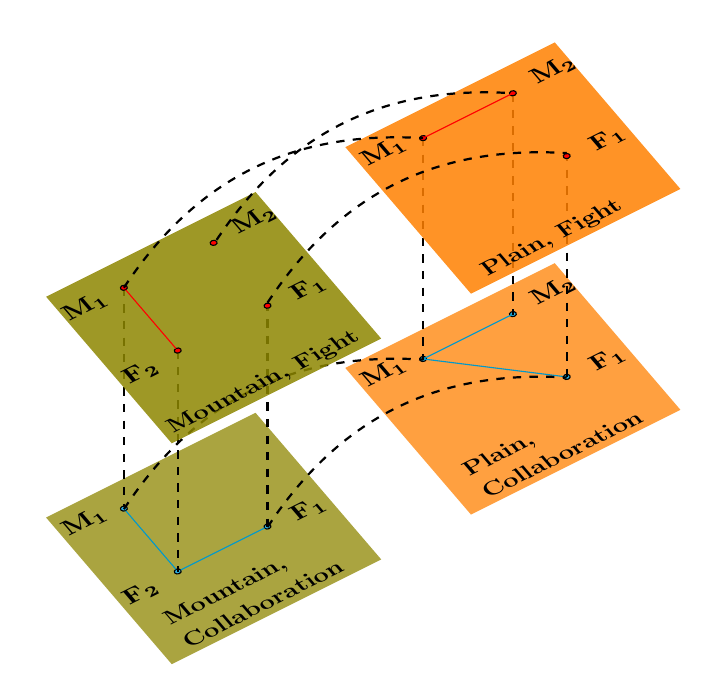
\begin{tikzpicture}[scale=0.38,every node/.style={minimum size=1cm},on grid]

	\node [mybox, scale=1.0] at (10.5, 2) (box){%
		\begin{minipage}{0.6\textwidth}
			
    	\end{minipage}
	};
	
	
	% etage 2
	\begin{scope}[
		yshift=-210,
		every node/.append style={yslant=\yslant,xslant=\xslant},
		yslant=\yslant,xslant=\xslant
	] 
		%\draw[black, dashed, thin] (0,0) rectangle (7,7); 
		\fill[olive,fill opacity=.75] (0,0) rectangle (7,7);
		
		\fill[orange,fill opacity=.75] (10,0) rectangle (17,7);
		%\draw[black, dashed, thin] (10,0) rectangle (17,7); 
		
		\draw[fill=echoreg]  %foret, collabo
			(5,3) node(111){} circle (.1) %A
			(2,3) circle (.1) %B
			(2,6) circle (.1); %C
			%(5,5) circle (.1); %D
		
		\draw[fill=echoreg]  %plaine, collabo
			(15,3) node(111){} circle (.1) %A
			%(12,2) circle (.1) %B
			(12,6) circle (.1) %C
			(15,6) circle (.1); %D
		 
		\draw[ thin, color=echodrk]%foret collab
			(2,5.9) to (2,3.1); %C->B
		\draw[ thin, color=echodrk]
			(2.1,3) to (4.9,3);%B->A
		
		\draw[thin, color=echodrk]%plaine collab
			(12,6) to (15,3);%C->A
		\draw[thin, color=echodrk]
			(12,6) to (15,6);
			
		\fill[black]
			(0.5,1.5) node[right, scale=.7] {\bf \large Mountain,} 	
			(0.5,0.5) node[right, scale=.7] {\bf \large Collaboration}
			(5.1,2.9) node[right,scale=.9]{$\mathbf{F_1}$}
			(1.9,2.9) node[left,scale=.9]{$\mathbf{F_2}$}
			(2,6.2) node[left,scale=.9]{$\mathbf{M_1}$};
			%(5.2,5.1) node[right,scale=.7]{\bf D}; 
			
		\fill[black]
			(10.5,1.5) node[right, scale=.7] {\bf \large Plain,}
			(10.5,0.5) node[right, scale=.7] {\bf \large Collaboration}
			(15.1,2.9) node[right,scale=.9]{$\mathbf{F_1}$}
			%(11.9,1.9) node[left,scale=.7]{\bf B}
			(12,6.2) node[left,scale=.9]{$\mathbf{M_1}$}
			(15.2,6.1) node[right,scale=.9]{$\mathbf{M_2}$}; 
		
		
	\end{scope}
	
	% Interlayer crossconnections
	% vertical
	\draw[thick,  dashed, decorate] (3.2, 4.7) to (3.2, -2.8);%A
	\draw[thick, dashed, decorate] (.2,3.1) to (.2,-4.3);%B
	\draw[thick,  dashed, decorate] (-1.6, 5.2) to (-1.6, -2.1);%C
	
1	\draw[thick,  dashed, decorate] (13.2,9.7) to (13.2, 2.2);%A
	\draw[thick, dashed, decorate] (11.4,11.7) to (11.4,4.3);%D
	\draw[thick,  dashed, decorate] (8.4, 10.2) to (8.4, 2.8);%c
	
	%horizontal
	
	
	\draw[thick, dashed, decorate] (-1.6,-2.2) to[bend left] (8.4,2.8);
	\draw[thick, dashed, decorate] (3.2,-2.8) to[bend left] (13.2,2.2);
	
	
	% etage 1
	\begin{scope}[
		yshift=0,
		every node/.append style={yslant=\yslant,xslant=\xslant},
		yslant=\yslant,xslant=\xslant
	]
		\fill[olive,fill opacity=.85] (0,0) rectangle (7,7); 
		%\draw[black, dashed, thin] (0,0) rectangle (7,7); 
		
		\fill[orange,fill opacity=.85] (10,0) rectangle (17,7);
		%\draw[black, dashed, thin] (10,0) rectangle (17,7); 
		
		\draw [fill=red]
			(5,3) node(111){} circle (.1)%A %foret, combat
			(2,3) circle (.1)%B
			(2,6) circle (.1)%C
			(5,6) circle (.1);%D

		\draw[fill=red]  
			(15,3) node(111){} circle (.1) %A % plaine combat
			%(12,2) circle (.1) %B
			(12,6) circle (.1) %C
			(15,6) circle (.1); %D
		
		\draw[thin, color=red]%foret combat
			(2,3.1) to (2,5.9);%B->C
			
		\draw[thin, color=red]%plaine combat
			(12,6) to (15,6);%C->D
		
		
		\fill[black]
			(0,0.5) node[right, scale=0.7] {\bf \large Mountain, Fight}
			(5.1,2.9) node[right,scale=0.9]{$\mathbf{F_1}$}
			(1.9,2.9) node[left,scale=0.9]{$\mathbf{F_2}$}
			(1.9,6) node[left,scale=0.9]{$\mathbf{M_1}$}
			(5.2,6.1) node[right,scale=0.9]{$\mathbf{M_2}$}; 
			
		\fill[black]
			(10.5,0.5) node[right, scale=.7] {\bf \large Plain, Fight}
			(15.1,2.9) node[right,scale=.9]{$\mathbf{F_1}$}
			%(11.9,1.9) node[left,scale=.7]{\bf B}
			(12,6.2) node[left,scale=.9]{$\mathbf{M_1}$}
			(15.2,6.1) node[right,scale=.9]{$\mathbf{M_2}$};
			
	\end{scope} 
	
	%interlayer
	\draw[thick, dashed, decorate] (-1.6,5.2) to[bend left] (8.4,10.2);%C
	\draw[thick, dashed, decorate] (3.2,4.7) to[bend left] (13.2,9.7);%A
	\draw[thick, dashed, decorate] (1.5,6.8) to[bend left] (11.4,11.7);%D
\end{tikzpicture}
\caption{The multilayer graph of relationships between monkeys. Red link between $M_1$ and $F_2$ means that the two monkeys have been fighting in the forest. The dotted links means that the nodes-layers are from the same nodes.}
\label{multimonkeys}
\end{center}
\end{figure}

\subsubsection{Stream graphs}
From the beginning, we added a link between two monkeys if they have been in contact, but we do not know anything about the times of existence of these contacts. We can use the stream graph to model this.

A {\em stream graph}~\cite{stream} is a set of four sets $S=(T,W,V,E)$.\\
$T$ is the time interval of study, $V$ is the set of nodes. The {\em time-nodes} set $W \subseteq T \times V$ describes the existence of nodes depending on the time: $(t,v) \in W$ means that the node $v$ appears at $t$. $E_M \subseteq T \times V \times V$ contain all the links and their time of existence.

Given nodes $u$ and $v$, we call $T_u$ the set of times at which $u$ appears, and $T_uv$ the set of time at which the link $(u,v)$ appears.

\begin{equation}
\begin{array}{rcl}
T_u&=&\{t, (t,u) \in W \}\\
T_{uv}&=&\{t, (t,uv)\in E \} 
\end{array}
\end{equation}

In the \cref{exmonkeystream}, we give an example of stream graph for the monkey population. We look at a place (let's say the forest) and we put a link between two monkeys when they interact.

\begin{figure}
\centering
	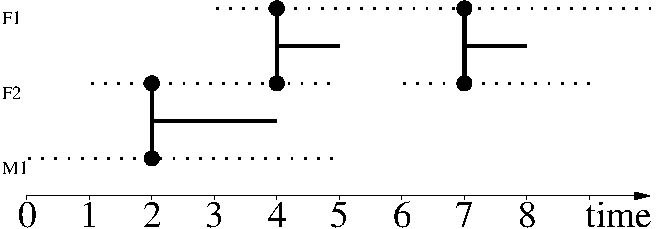
\includegraphics[width=0.5\textwidth]{img/ext.pdf}
	\caption{Example of stream graph describing interactions between monkeys in the forest. $F_1$ arrives at $t=3$, and interacts with $F_2$ at $t \in[4,5]\cup [7,8]$. $F_2$ and $M_1$ interact between $t=2$ and $4$.}
	\label{exmonkeystream}
\end{figure}

The stream graph model does not require, as for other temporal graph models, to discretize the time. Several notions have been designed on \cite{stream} from the model of the graph notions. Among them, we can find the number of nodes, the density, the uniformity, the compacity , the degree, the betweenness centrality, path and distances.

\subsection{Definition of the multilayer stream graph}
%
We now gather the notion of multilayer graphs and stream graphs to capture both structure and temporal subtleties.

We define a multilayer stream graph (MSG) as a tuple $S_M = (T,T_M,V,W_M,E_M,{\cal L})$, such that $T$ and $V$ are, respectively, a time interval and a set of nodes, just like for stream graphs \cite{stream}.
    
    As for multilayer graphs \cite{mlkiv}, ${\cal L}$ is a set of $d$ {\em aspects}; ${\cal L} = \{L_i\}_{i=1}^d$, and an element $\alpha_i$ of $L_i$ is named {\em elementary layer}. An element of $L=L_1\times \dots \times L_d$ is named {\em layer}.

	$T_M$ is a set of intervals of $T$ so for that each layer $\alpha$, $T_{\alpha}$ is the interval at which the layer exists. For each $t$ in $T$, $\exists \alpha \in L | t \in T_{\alpha}$. At each time of $T$, at least one layer of $L$ exists.

	$W_M \subseteq T\times V \times (L_1 \times \dots \times L_d)$ represents the existing points on layers with respect to time. For each element $(t,u,\alpha)$ of $W_M$, $t$ must be in the interval of existence of $\alpha$.

   $E_M \subseteq T\times V_M \otimes V_M$ are the links appearing with respect to time,  $V_M = \{ (u,\alpha), u\in V, \alpha \in L\}$. The elements of $V_M$ are named {\em node-layer}. A link can not appear outside the time of existence of the two node-layers.
   
   We give an example of modelisation for the imaginary multilayer stream graph of relationships between monkeys, \cref{multistreamMonkeys}.
   \begin{figure}[h]
   	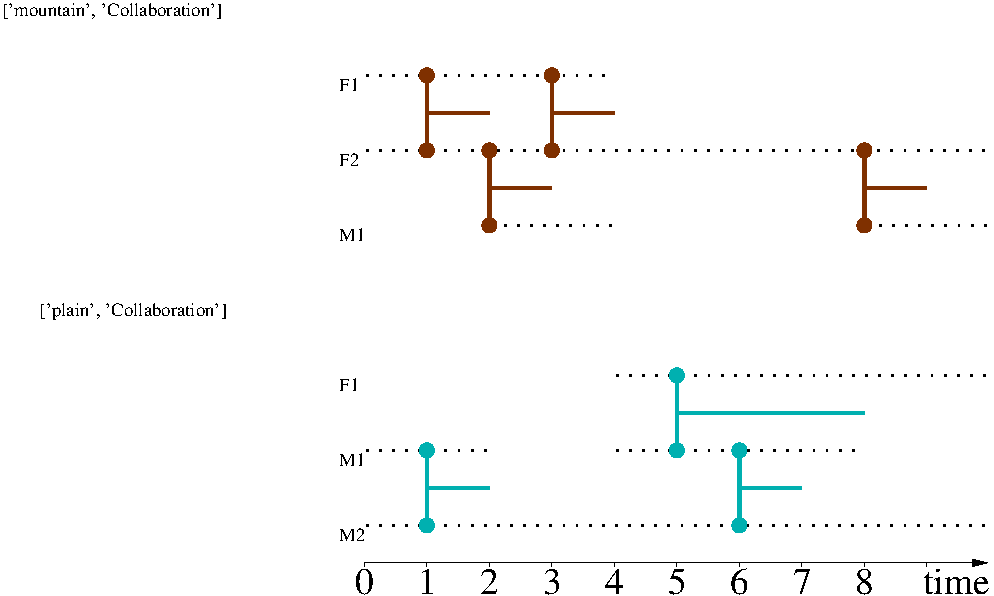
\includegraphics[width=0.8\textwidth]{img/monkeymls.pdf}
   	\caption{An example of the 2-layers stream graph of monkeys, collaborating in mountain or in plain. $F_1$ is in [mountain, collaboration] between $t=0$ and $t=4$ and then goes to [plain,collaboration]. It collaborates with $F_2$ at $t\in [1,2]\cup[3,4]$: $\{(t,F_1,[\text{mountain,collaboration}],F_2,[\text{mountain,collaboration}]),t\in [1,2]\cup[3,4]\} \subset E_M$.}
   	\label{multistreamMonkeys}
   \end{figure}
   
%
\subsection{Basic notions}
%
\subsubsection{Extractions}

We built a object containing both the temporal and structural aspect, we now explain how to do the reverse operation, how we can extract some stream graphs, multilayer graphs and graphs from a multilayer stream graph.

\begin{definition}[Induced multilayer graph]
    The {\em induced multilayer graph by the set } $\tau \subseteq T$ is a multilayer graph $M_I(S_M)=(V_{M,I}, E_{M,I}, V,L)$ which gathers all the layers, nodes-layers and links existing during a time of $\tau$.
    \begin{align*}
    	V_{M,I} = \{ v \in V | \exists t \in \tau, (t,v) \in V_M\}\\
    	E_{M,I} = \{((v,\alpha),(w,\beta)) \in (V\times L)\otimes (V\times L) | \exists t \in \tau , (t,v,\alpha,w,\beta) \in E_M \} \\
    \end{align*}
    In our example of monkeys, the lower part of \cref{multimonkeys} is the induced multilayer stream graph of the multilayer stream graph represented \cref{multistreamMonkeys}.
\end{definition}

In the case of $\tau={t}$, we call the induced multilayer graph the {\em multilayer graph at time} $t$.

We also extract sub-stream graph and sub-multilayer stream graphs, using the properties of the layers.

\begin{definition}[Intralayer sub stream graph]	
	For each layer $\alpha \in L_1 \times \dots \times L_d$, the {\em intralayer stream graph} $S^{\alpha}$ is the stream graph $S^{\alpha}=(T_{\alpha},V^{\alpha},W^{\alpha},E^{\alpha})$ such that $ T_{\alpha} \in T_M$ is the existence interval of $\alpha$. $V^{\alpha}$ is the set of node-layers in the layer $\alpha$ and $W^{\alpha}$ represents their times of appearance in the layer $\alpha$. $E^{\alpha}$ is the subset $E_M$ containing only the edges between node-layers of $\alpha$.
	\end{definition}
	
	
	\begin{definition}[Interlayer stream graphs]		
	Given a doublet of layers $\alpha, \beta \in L_1\times \dots\times L_d$, the {\em interlayer stream graph} is the bipartite stream graph $S^{(\alpha,\beta)} = (T^{\alpha,\beta}, V^{\alpha,\beta},W^{\alpha,\beta},E^{\alpha,\beta})$ such that: $T^{\alpha,\beta}=T^{\alpha}\cap T^{\beta}$ is the interval of time in wich $\alpha$ and $\beta$ appear simultaneously. $V^{\alpha,\beta}$ are all the node-layers of the multilayer stream graph which are in the layers $\alpha$ and $\beta$, $W^{\alpha,\beta}$ describes all their intervals of existence. Finally, $E^{\alpha,\beta}$ are the not-oriented links between node-layers of layers $\alpha$ and $\beta$ with their times of existence.
	\end{definition}
	
\begin{definition}[Underlying stream graph]
	The underlying stream graph $S_U(S_M)$ $S_M$ is  $(T,V_M,W_M,E_M)$. It's the stream graph in which the nodes are the nodes-layers from $S_M$. There is a link between two nodes if there is a link between two corresponding node-layers.
\end{definition}
	
	\begin{definition}[Aggregated stream graph]
		
		The aggregated stream graph $S_A(S_M)=(T,V,W_A,E_A)$ has the same interval of study $T$ than $S_M$. Its nodes are the same as in $S_M$ (the set $V$). Their times of existence are the union of their time of existence on the different layers: $T_u = \bigcup_{\alpha \in L} T_{u,\alpha}$ and $W_A=\bigcup_{u\in V} T_u\times\{u\}$. An edge exists between two nodes of $S_A(S_M)$ if it exists a the same time between two correspondent node-layers of $S_M$:  $E_A = \{(t,u,v)| \exists (\alpha,\beta) \in L^2, (t,(u,\alpha),(v,\beta)) \in E_M \}$.
	\end{definition}

\subsection{Density}
%
In a classical graph $G=(V,E)$, the density is the rate of connections: $\delta(G)= \frac{|E|}{|V|^2}$ if the graph is directed, and  $\delta(G)= \frac{2|E|}{|V|(|V|-1)}$ if it's not directed. We focus on the undirected multilayer stream graphs.

\begin{definition}[Density of a multilayer stream graph]	Let's call $C \in T \times V_M\times V_M$ the set of ``possible links'' in the multilayer stream graph. If some links are implied (the links between the nodes-layers from the same nodes), they are not in $C$. 
	
	The density is then written as follows:
	\[
		\delta_M (M) 
		%= \frac{\int_{t\in T}|E_M,t|}{\int_{t\in T}|C_t|} 
		= \frac{\sum_{(u,\alpha)(v,\beta) \in E_M}|T_{(u,\alpha)(v,\beta)}|}{|C|}
	\]
\end{definition}	
	


\subsection{Centralities}
%
A centrality is a measure that quantifies the influence of elements of a graph on the whole graph. In a classical graph, we measure the importance of nodes with the degree, the page-ranking \cite{pr}, with the betweenness centrality \cite{btw}, among a lot of others. But we can also compute betweenness centrality on links, for instance to know which links we have to remove to break a connected component.

In our case, we have nodes, layers, node-layers, and links. This means that the measures become more complex and more diverse.
%
\subsubsection{Centrality of nodes and the paths}
%
In classical graph, the centrality of the nodes describe how much we will encounter a node while browsing a graph. They are different way to browse a graph: the random walk, the contamination models, the shortest path, etc. In the stream graph, the notions are more numerous: we can compute random walks, but with different laws of probabilities of transition, same for the contamination. We can look for the shortest paths (with the less transitions possible) but the fastest paths (the ones that take less time), the foremost paths (the ones that arrives the earliest starting from a certain time), and we can combine those notions.



\subsubsection{Centrality in layers}

Two types of groups of layers are preponderant in multilayer graphs, the superimposed layers and the juxtaposed layers, and we define centralities for the two types of layers.

The {\bf superimposed layers}: in this group of layers, nodes can appear on all layers. It is the case for layers describing to diverse types of relationships. If two different node-layers are from different nodes and different superimposed layers, we don't have a link between those two node-layers. A relevant way to study those layers is be to compare them.

The {\bf juxtaposed layers} forms a partition of the nodes. For instance, they can model people from different classes in the same school. A relevant way to deal with those layers is to study the interactions between them.


\subsubsection{Centrality of times}
%

\subsubsection{Experimental centralities: random walk}
%

\subsection{Implementation and complexity}
%
\subsection{Autonomous Systems}
%

\section{Datasets and results}
%
\subsection{Two datasets}
%
\subsubsection{Classes in an high school: a social multilayer stream graph}
%
\subsubsection{Civil airlines in US: an application to transportation}
%
\subsection{Analysis}
%

% ---- Bibliography ----
%
\begin{thebibliography}{6}
%

%\bibitem {smit:wat}
%Smith, T.F., Waterman, M.S.: Identification of common molecular subsequences.
%J. Mol. Biol. 147, 195?197 (1981). \url{doi:10.1016/0022-2836(81)90087-5}

\bibitem{stream}
Latapy M.,Viard T.,Magnien C.: Stream graphs and link streams for the modeling
of interactions over time. (October 2018) In: Social Network Analysis and Mining, vol.8. arXiv preprint arXiv:1710.04073. \url{doi:https://doi.org/10.1007/s13278-018-0537-7}

\bibitem{mlkiv}
Kivela M., Arenas A., Barthelemy M., Gleeson J.P., Moreno Y., Porter M.A.: Multilayer Networks. (2014) In: Journal of Complex Networks",vol.2.

\bibitem{mldd}
De Domenico M., Sol\'e-Ribalta A., Cozzo E., Kivel\"a M., Moreno Y., Porter M.A., G\'omez S., Arenas A.: Mathematical Formulation of Multilayer Networks.(2013). In: Phys. Rev. X. doi:10.1103/PhysRevX.3.041022

%page rank
\bibitem{pr}
Brin S., Page L.: The anatomy of a large-scale hypertextual web search engine (1998). In: Proceedings of the Seventh World Wide Web Conference

%betweenness centrality
\bibitem{btw}
Brandes U.: A faster algorithm for betweenness centrality (2001). In: Journal of mathematical sociology.
% --------------------------------------------------



\end{thebibliography}
\end{document}
